\documentclass[a4paper,12pt,twoside]{memoir}

% Castellano
\usepackage[spanish,es-tabla]{babel}
\selectlanguage{spanish}
\usepackage[utf8]{inputenc}
\usepackage[T1]{fontenc}
\usepackage{lmodern} % scalable font
\usepackage{microtype}
\usepackage{placeins}
\usepackage{eurosym} % símbolo del euro
\usepackage{pdflscape} % landscape pages  
 
\RequirePackage{longtable,booktabs}
\RequirePackage[table]{xcolor}
\RequirePackage{xtab}
\RequirePackage{multirow}

% Links
\usepackage[colorlinks]{hyperref}
\hypersetup{
	allcolors = {red}
}

% Ecuaciones
\usepackage{amsmath}

% Rutas de fichero / paquete
\newcommand{\ruta}[1]{{\sffamily #1}}

% Párrafos
\nonzeroparskip

% Huérfanas y viudas
\widowpenalty100000
\clubpenalty100000

% Evitar solapes en el header
\nouppercaseheads

% Imagenes
\usepackage{graphicx}
\newcommand{\imagen}[2]{
	\begin{figure}[!h]
		\centering
		\includegraphics[width=0.9\textwidth]{#1}
		\caption{#2}\label{fig:#1}
	\end{figure}
	\FloatBarrier
}

\newcommand{\imagenflotante}[2]{
	\begin{figure}%[!h]
		\centering
		\includegraphics[width=0.9\textwidth]{#1}
		\caption{#2}\label{fig:#1}
	\end{figure}
}

\newcommand{\imagengrande}[3]{
	\begin{figure}[H]
		\centering
		\includegraphics[width=#1\textwidth]{#2}
		\caption{#3}\label{fig:#2}
	\end{figure}
}



% El comando \figura nos permite insertar figuras comodamente, y utilizando
% siempre el mismo formato. Los parametros son:
% 1 -> Porcentaje del ancho de página que ocupará la figura (de 0 a 1)
% 2 --> Fichero de la imagen
% 3 --> Texto a pie de imagen
% 4 --> Etiqueta (label) para referencias
% 5 --> Opciones que queramos pasarle al \includegraphics
% 6 --> Opciones de posicionamiento a pasarle a \begin{figure}
\newcommand{\figuraConPosicion}[6]{%
  \setlength{\anchoFloat}{#1\textwidth}%
  \addtolength{\anchoFloat}{-4\fboxsep}%
  \setlength{\anchoFigura}{\anchoFloat}%
  \begin{figure}[#6]
    \begin{center}%
      \Ovalbox{%
        \begin{minipage}{\anchoFloat}%
          \begin{center}%
            \includegraphics[width=\anchoFigura,#5]{#2}%
            \caption{#3}%
            \label{#4}%
          \end{center}%
        \end{minipage}
      }%
    \end{center}%
  \end{figure}%
}

%
% Comando para incluir imágenes en formato apaisado (sin marco).
\newcommand{\figuraApaisadaSinMarco}[5]{%
  \begin{figure}%
    \begin{center}%
    \includegraphics[angle=90,height=#1\textheight,#5]{#2}%
    \caption{#3}%
    \label{#4}%
    \end{center}%
  \end{figure}%
}
% Para las tablas
\newcommand{\otoprule}{\midrule [\heavyrulewidth]}
%
% Nuevo comando para tablas pequeñas (menos de una página).
\newcommand{\tablaSmall}[5]{%
 \begin{table}[!h]
  \begin{center}
   \rowcolors {2}{gray!35}{}
   \begin{tabular}{#2}
    \toprule
    #4
    \otoprule
    #5
    \bottomrule
   \end{tabular}
   \caption{#1}
   \label{tabla:#3}
  \end{center}
 \end{table}
}

%
%Para el float H de tablaSmallSinColores
\usepackage{float}

%
% Nuevo comando para tablas pequeñas (menos de una página).
\newcommand{\tablaSmallSinColores}[5]{%
 \begin{table}[H]
  \begin{center}
   \begin{tabular}{#2}
    \toprule
    #4
    \otoprule
    #5
    \bottomrule
   \end{tabular}
   \caption{#1}
   \label{tabla:#3}
  \end{center}
 \end{table}
}

\newcommand{\tablaApaisadaSmall}[5]{%
\begin{landscape}
  \begin{table}
   \begin{center}
    \rowcolors {2}{gray!35}{}
    \begin{tabular}{#2}
     \toprule
     #4
     \otoprule
     #5
     \bottomrule
    \end{tabular}
    \caption{#1}
    \label{tabla:#3}
   \end{center}
  \end{table}
\end{landscape}
}

%
% Nuevo comando para tablas grandes con cabecera y filas alternas coloreadas en gris.
\newcommand{\tabla}[6]{%
  \begin{center}
    \tablefirsthead{
      \toprule
      #5
      \otoprule
    }
    \tablehead{
      \multicolumn{#3}{l}{\small\sl continúa desde la página anterior}\\
      \toprule
      #5
      \otoprule
    }
    \tabletail{
      \hline
      \multicolumn{#3}{r}{\small\sl continúa en la página siguiente}\\
    }
    \tablelasttail{
      \hline
    }
    \bottomcaption{#1}
    \rowcolors {2}{gray!35}{}
    \begin{xtabular}{#2}
      #6
      \bottomrule
    \end{xtabular}
    \label{tabla:#4}
  \end{center}
}

%
% Nuevo comando para tablas grandes con cabecera.
\newcommand{\tablaSinColores}[6]{%
  \begin{center}
    \tablefirsthead{
      \toprule
      #5
      \otoprule
    }
    \tablehead{
      \multicolumn{#3}{l}{\small\sl continúa desde la página anterior}\\
      \toprule
      #5
      \otoprule
    }
    \tabletail{
      \hline
      \multicolumn{#3}{r}{\small\sl continúa en la página siguiente}\\
    }
    \tablelasttail{
      \hline
    }
    \bottomcaption{#1}
    \begin{xtabular}{#2}
      #6
      \bottomrule
    \end{xtabular}
    \label{tabla:#4}
  \end{center}
}

%
% Nuevo comando para tablas grandes sin cabecera.
\newcommand{\tablaSinCabecera}[5]{%
  \begin{center}
    \tablefirsthead{
      \toprule
    }
    \tablehead{
      \multicolumn{#3}{l}{\small\sl continúa desde la página anterior}\\
      \hline
    }
    \tabletail{
      \hline
      \multicolumn{#3}{r}{\small\sl continúa en la página siguiente}\\
    }
    \tablelasttail{
      \hline
    }
    \bottomcaption{#1}
  \begin{xtabular}{#2}
    #5
   \bottomrule
  \end{xtabular}
  \label{tabla:#4}
  \end{center}
}



\definecolor{cgoLight}{HTML}{EEEEEE}
\definecolor{cgoExtralight}{HTML}{FFFFFF}

%
% Nuevo comando para tablas grandes sin cabecera.
\newcommand{\tablaSinCabeceraConBandas}[5]{%
  \begin{center}
    \tablefirsthead{
      \toprule
    }
    \tablehead{
      \multicolumn{#3}{l}{\small\sl continúa desde la página anterior}\\
      \hline
    }
    \tabletail{
      \hline
      \multicolumn{#3}{r}{\small\sl continúa en la página siguiente}\\
    }
    \tablelasttail{
      \hline
    }
    \bottomcaption{#1}
    \rowcolors[]{1}{cgoExtralight}{cgoLight}

  \begin{xtabular}{#2}
    #5
   \bottomrule
  \end{xtabular}
  \label{tabla:#4}
  \end{center}
}




\graphicspath{ {./img/} }

% Capítulos
\chapterstyle{bianchi}
\newcommand{\capitulo}[2]{
	\setcounter{chapter}{#1}
	\setcounter{section}{0}
	\setcounter{figure}{0}
	\setcounter{table}{0}
	\chapter*{#2}
	\addcontentsline{toc}{chapter}{#2}
	\markboth{#2}{#2}
}

% Apéndices
\renewcommand{\appendixname}{Apéndice}
\renewcommand*\cftappendixname{\appendixname}

\newcommand{\apendice}[1]{
	%\renewcommand{\thechapter}{A}
	\chapter{#1}
}

\renewcommand*\cftappendixname{\appendixname\ }

% Formato de portada
\makeatletter
\usepackage{xcolor}
\newcommand{\tutor}[1]{\def\@tutor{#1}}
\newcommand{\course}[1]{\def\@course{#1}}
\definecolor{cpardoBox}{HTML}{E6E6FF}
\def\maketitle{
  \null
  \thispagestyle{empty}
  % Cabecera ----------------
\noindent
\includegraphics[width=\textwidth]{cabecera}\vspace{1cm}%
  \vfill
  % Título proyecto y escudo informática ----------------
  \colorbox{cpardoBox}{%
    \begin{minipage}{.8\textwidth}
      \vspace{.5cm}\Large
      \begin{center}
      \textbf{TFG del Grado en Ingeniería Informática}\vspace{.6cm}\\
      \textbf{\LARGE\@title{}}
      \end{center}
      \vspace{.2cm}
    \end{minipage}

  }%
  \hfill\begin{minipage}{.20\textwidth}
    
\includegraphics[width=\textwidth]{escudoInfor}
  \end{minipage}
  \vfill
  % Datos de alumno, curso y tutores ------------------
  \begin{center}%
  {%
    \noindent\LARGE
    Presentado por \@author{}\\ 
    en Universidad de Burgos --- \@date{}\\
    Tutor: \@tutor{}\\
  }%
  \end{center}%
  \null
  \cleardoublepage
  }
\makeatother

\newcommand{\nombre}{Francisco Martín Vargas} %%% cambio de comando
\newcommand{\nombretutor}{César Represa Pérez}

% Datos de portada
\title{{\Huge DomoCamera}\\[0.25cm]Entorno domótico para la monitorización de cámaras desde Android. \\Documentación Técnica}
\author{\nombre}
\tutor{\nombretutor}
\date{\today}

\begin{document}

\maketitle



\cleardoublepage



%%%%%%%%%%%%%%%%%%%%%%%%%%%%%%%%%%%%%%%%%%%%%%%%%%%%%%%%%%%%%%%%%%%%%%%%%%%%%%%%%%%%%%%%



\frontmatter


\clearpage

% Indices
\tableofcontents

\clearpage

\listoffigures

\clearpage

\listoftables

\clearpage

\mainmatter

\appendix

\apendice{Plan de Proyecto Software}

\section{Introducción}

\section{Planificación temporal}

\section{Estudio de viabilidad}

\subsection{Viabilidad económica}

\subsection{Viabilidad legal}



\apendice{Especificación de Requisitos}

\section{Introducción}

La Especificación de Requisitos Software (ERS) pretende obtener una descripción completa del comportamiento del sistema que va a ser desarrollado. 
En él se anotan las necesidades del producto (tanto para usuario, como para cliente), además de definirse los requerimientos del sistema. 
Incluye la totalidad de los casos de uso de las interacciones del usuario final con el software.
Este documento sirve de medio de comunicación entre todas las partes (desarrolladores, clientes y usuarios finales).\\

Según el estándar IEEE-STD-830-1998 \cite{ieee830} un ERS debe presentar las siguientes características:

\begin{itemize}
\item
	\textbf{Correcto}\\
	Un ERS es correcto si, y sólo si, cada requisito declarado se encuentra en el software
\item
	\textbf{Inequívoco}\\
	Un SRS es inequívoco si, y sólo si, cada requisito declarado tiene una sola interpretación.
\item
	\textbf{Completo}\\
	Un SRS es completo si, y sólo si, incluye: 
		\begin{itemize}
		\item
			Requisitos relacionados a funcionalidad, desarrollo, restricciones
de diseño, atributos e interfaces externas.
		\item
			 Definiciones de las respuestas del software a todos los posibles datos de la entrada del sistema y a toda clase de situaciones.
		\item
			 Tener todas las etiquetas llenas y bien referencias. 
		\end{itemize}
\item
	\textbf{Consistente}\\
	Un SRS debe ser coherente con los requerimientos del ERS y con todos los documentos de distinto nivel.
\item
	\textbf{Delinear que tiene importancia y/o estabilidad}\\
	Un SRS debe delinear la importancia y/o estabilidad de cada requisito. Cada requisito mantiene un identificador que identifica la importancia o estabilidad de dicho requisito. 
\item
	\textbf{Comprobable}\\
	Un SRS es comprobable si, y sólo si, cada requisito declarado es verificable. 
	Un requisito es verificable si, y sólo si, allí existe algún método finito para verificar que el producto del software reúne el requisito.
\item
	\textbf{Modificable}\\
	Un SRS es modificable si, y sólo si, su estructura y estilo permite cualquier cambio a los requisitos fácilmente, completamente y de forma consistente mientras conserva la estructura y estilo.
\item
	\textbf{Identificable}\\
	Un SRS es identificable si el origen de los requisitos es claro y facilita las referencias en el desarrollo futuro o documentación del mismo. 
\end{itemize}

\section{Objetivos generales}

Se pretende cumplir los objetivos siguientes:

\begin{itemize}
\tightlist
\item
  Desarrollar una aplicación para el entorno Android que permita la monitorización de cámaras dispuestas en un hogar.
\item
  Desarrollar y desplegar un servidor que gestione el entorno domótico (la conexión con las cámaras y con la aplicación Android).
\item
  Facilitar al usuario la monitorización mediante una interfaz fácil y sencilla.
\item
  Utilizar dispositivos de bajo consumo.
\end{itemize}



\section{Catalogo de requisitos}

En este apartado se presentarán los requisitos del sistema, tanto los funcionales como los no funcionales.

\subsection{Requisitos funcionales}

\begin{itemize}
	\item
		\textbf{RF-1 Gestión de cámaras:} 
			El sistema debe de ser capaz de realizar la gestión de las cámaras.
		\begin{itemize}
			\item
				\textbf{RF-1.1 Añadir cámara:}
					El usuario debe de ser capaz de añadir una cámara con un nombre que la identifique, la ip de acceso a la cámara y un puerto de envío. 
					\begin{itemize}
						\item
							\textbf{RF-1.1.1 Conectar cámara:}
								El servidor debe de ser capaz de conectarse a una cámara a petición del usuario.
					\end{itemize}
			\item
				\textbf{RF-1.2 Eliminar cámara:}
					El usuario debe de ser capaz de eliminar una cámara existente en el sistema.
		\end{itemize}
		
	\item
		\textbf{RF-2 Gestión de la conexión aplicación-servidor:} 
			El sistema debe de ser capaz de realizar la gestión de la conexión del servidor con la aplicación.
		\begin{itemize}
			\item
				\textbf{RF-2.1 Conectar al servidor:}
					El usuario debe de ser capaz de conectarse al servidor a través de la ip del servidor y el puerto de escucha. 
			\item
				\textbf{RF-2.2 Desconectar del servidor:}
					El usuario debe de ser capaz de desconectarse del servidor.
		\end{itemize}
		
	\item
		\textbf{RF-3 Monitorización de las cámaras:} 
			El usuario debe ser capaz de poder monitorizar todas las cámaras conectadas al sistema.
			\begin{itemize}
			\item
				\textbf{RF-3.1 Visualizar imagen:}
					El usuario debe de ser capaz de visualizar la imagen procedente de las cámaras.
		\end{itemize}
	
	\item
		\textbf{RF-4 Gestión del servidor:} 
			El sistema debe de ser capaz de realizar la gestión del servidor.
		\begin{itemize}
			\item
				\textbf{RF-4.1 Iniciar servidor:}
					El usuario debe de ser capaz de iniciar el servidor.
			\item
				\textbf{RF-4.2 Parar servidor:}
					El usuario debe de ser capaz de parar el servidor.
		\end{itemize}
\end{itemize}



\subsection{Requisitos no funcionales}

\begin{itemize}
	\item
		\textbf{RNF-1 Usabilidad:}
			La aplicación debe mantener una interfaz de usuario intuitiva, debe parecerse lo suficiente a otras aplicaciones del mismo entorno para que la curva de aprendizaje sea lo suficientemente corta como para la no necesidad de un tutorial.
	\item
		\textbf{RNF-2 Rendimiento:} 
			El sistema debe mantener una cierta fluidez, no se deben presentar fallos o paradas del sistema, independientemente del dispositivo utilizado.
	\item
		\textbf{RNF-3 Disponibilidad:} 
			El servidor debe ser accesible en cualquier momento desde la aplicación mientras este haya sido iniciado. 
			Además la aplicación debe estar disponible para su uso independientemente del momento de acceso.
	\item
		\textbf{RNF-4 Estabilidad:} 
			El sistema debe ser estable, debe mantener un nivel bajo de fallos y ser capaz de enmascarar los mismos al usuario.
	\item
		\textbf{RNF-5 Robustez:} 
			El sistema debe ser capaz de soportar circunstancias no anticipadas sin que se produzca una caída o fallo del sistema.
	\item
		\textbf{RNF-6 Fiabilidad (validez e integridad):} 
			El sistema debe mantener la validez de todas las acciones que se realizan en el mismo, mantenido la integridad de los datos.
	\item
		\textbf{RNF-7 Seguridad:} 
			El sistema debe mantener la seguridad de forma que no se comprometa la información del usuario.
	\item
		\textbf{RNF-8 Mantenibilidad:} 
			El sistema debe permitir la corrección de fallos, mejora de rendimiento (escalabilidad) o adaptaciones con facilidad.
	\item
		\textbf{RNF-9 Soporte:} 
			La aplicación debe dar soporte a dispositivos con versiones de Android iguales o superiores a Android 4.1 (Jelly Bean).
\end{itemize}



\section{Especificación de requisitos}

En este apartado vamos a mostrar los casos de uso de cada una de las acciones derivadas de los requisitos funcionales del proyecto.

\subsection{Caso de uso general}

\imagen{casoUsoGeneral}{Caso de uso general de la especificación de requisitos.}

\subsection{Actores}

El único  actor que actúa con el sistema es el usuario final.

\subsection{Casos de uso}

%CASO DE USO 1

\begin{longtable}[h!]{@{}ll@{}}
\toprule
\begin{minipage}[b]{0.23\columnwidth}\raggedright\strut
\textbf{CU-1}\strut
\end{minipage} & \begin{minipage}[b]{0.71\columnwidth}\raggedright\strut
\textbf{Gestión de cámaras}\strut
\end{minipage}\tabularnewline
\midrule
\endhead
\begin{minipage}[t]{0.23\columnwidth}\raggedright\strut
\textbf{Versión}\strut
\end{minipage} & \begin{minipage}[t]{0.71\columnwidth}\raggedright\strut
1.0\strut
\end{minipage}\tabularnewline
\begin{minipage}[t]{0.23\columnwidth}\raggedright\strut
\textbf{Autor}\strut
\end{minipage} & \begin{minipage}[t]{0.71\columnwidth}\raggedright\strut
\nombre\strut
\end{minipage}\tabularnewline
\begin{minipage}[t]{0.23\columnwidth}\raggedright\strut
\textbf{Requisitos asociados}\strut
\end{minipage} & \begin{minipage}[t]{0.71\columnwidth}\raggedright\strut
RF-1, RF-1.1, RF-1.1.1, RF-1.2\strut
\end{minipage}\tabularnewline
\begin{minipage}[t]{0.23\columnwidth}\raggedright\strut
\textbf{Descripción}\strut
\end{minipage} & \begin{minipage}[t]{0.71\columnwidth}\raggedright\strut
Permite al usuario gestionar sus cámaras.\strut
\end{minipage}\tabularnewline
\begin{minipage}[t]{0.23\columnwidth}\raggedright\strut
\textbf{Precondición}\strut
\end{minipage} & \begin{minipage}[t]{0.71\columnwidth}\raggedright\strut
El usuario debe encontrarse en la pestaña principal (home).\\
La aplicación debe estar conectada al servidor.\strut
\end{minipage}\tabularnewline
\begin{minipage}[t]{0.23\columnwidth}\raggedright\strut
\textbf{Acciones}\strut
\end{minipage} & \begin{minipage}[t]{0.71\columnwidth}\raggedright\strut
\begin{enumerate}
\def\labelenumi{\arabic{enumi}.}
\tightlist
\item
  Se listan todas las cámaras que están disponibles.
\item
  Para cada una de las cámaras se muestra un botón para poder acceder a ella.
\item
  Se muestra un menú en el que al pulsar podremos añadir o eliminar cámaras.
\end{enumerate}\strut
\end{minipage}\tabularnewline
\begin{minipage}[t]{0.23\columnwidth}\raggedright\strut
\textbf{Postcondición}\strut
\end{minipage} & \begin{minipage}[t]{0.71\columnwidth}\raggedright\strut
El número de cámaras mostrado es el mismo que el servidor y la aplicación tienen en sus bases de datos.\strut
\end{minipage}\tabularnewline
\begin{minipage}[t]{0.23\columnwidth}\raggedright\strut
\textbf{Excepciones}\strut
\end{minipage} & \begin{minipage}[t]{0.71\columnwidth}\raggedright\strut
\begin{itemize}
\tightlist
\item
  Error al cargar cámaras (mensaje).
\item
  No hay cámaras introducidas (pantalla vacía).
\end{itemize}\strut
\end{minipage}\tabularnewline
\begin{minipage}[t]{0.23\columnwidth}\raggedright\strut
\textbf{Importancia}\strut
\end{minipage} & \begin{minipage}[t]{0.71\columnwidth}\raggedright\strut
Alta\strut
\end{minipage}\tabularnewline
\bottomrule
\caption{CU-1 Gestión de cámaras.}
\end{longtable}

%CASO DE USO 2 ---------------------------------------------------------

\begin{longtable}[h!]{@{}ll@{}}
\toprule
\begin{minipage}[b]{0.23\columnwidth}\raggedright\strut
\textbf{CU-2}\strut
\end{minipage} & \begin{minipage}[b]{0.71\columnwidth}\raggedright\strut
\textbf{Añadir cámara}\strut
\end{minipage}\tabularnewline
\midrule
\endhead
\begin{minipage}[t]{0.23\columnwidth}\raggedright\strut
\textbf{Versión}\strut
\end{minipage} & \begin{minipage}[t]{0.71\columnwidth}\raggedright\strut
1.0\strut
\end{minipage}\tabularnewline
\begin{minipage}[t]{0.23\columnwidth}\raggedright\strut
\textbf{Autor}\strut
\end{minipage} & \begin{minipage}[t]{0.71\columnwidth}\raggedright\strut
\nombre\strut
\end{minipage}\tabularnewline
\begin{minipage}[t]{0.23\columnwidth}\raggedright\strut
\textbf{Requisitos asociados}\strut
\end{minipage} & \begin{minipage}[t]{0.71\columnwidth}\raggedright\strut
RF-1.1, RF-1.1.1\strut
\end{minipage}\tabularnewline
\begin{minipage}[t]{0.23\columnwidth}\raggedright\strut
\textbf{Descripción}\strut
\end{minipage} & \begin{minipage}[t]{0.71\columnwidth}\raggedright\strut
Permite al usuario añadir una cámara.\strut
\end{minipage}\tabularnewline
\begin{minipage}[t]{0.23\columnwidth}\raggedright\strut
\textbf{Precondición}\strut
\end{minipage} & \begin{minipage}[t]{0.71\columnwidth}\raggedright\strut
El usuario debe encontrarse en la pestaña principal (home).\\
La aplicación debe estar conectada al servidor.\strut
\end{minipage}\tabularnewline
\begin{minipage}[t]{0.23\columnwidth}\raggedright\strut
\textbf{Acciones}\strut
\end{minipage} & \begin{minipage}[t]{0.71\columnwidth}\raggedright\strut
\begin{enumerate}
\def\labelenumi{\arabic{enumi}.}
\tightlist
\item
  El usuario pulsa el botón del menú desplegable superior derecho.
\item
  El usuario elige la opción ``\textit{Añadir cámara}''.
\item
  El usuario rellena los campos \textit{nombre}, \textit{IP} y \textit{Puerto}.
\item
  El usuario pulsa el botón aceptar.
\end{enumerate}\strut
\end{minipage}\tabularnewline
\begin{minipage}[t]{0.23\columnwidth}\raggedright\strut
\textbf{Postcondición}\strut
\end{minipage} & \begin{minipage}[t]{0.71\columnwidth}\raggedright\strut
Se ha añadido una nueva cámara en la pantalla principal y la información ha sido almacenada en las bases de datos.\strut
\end{minipage}\tabularnewline
\begin{minipage}[t]{0.23\columnwidth}\raggedright\strut
\textbf{Excepciones}\strut
\end{minipage} & \begin{minipage}[t]{0.71\columnwidth}\raggedright\strut
\begin{itemize}
\tightlist
\item
  Error al en la conexión (mensaje).
\item
  Cámara ya existente (mensaje).
\end{itemize}\strut
\end{minipage}\tabularnewline
\begin{minipage}[t]{0.23\columnwidth}\raggedright\strut
\textbf{Importancia}\strut
\end{minipage} & \begin{minipage}[t]{0.71\columnwidth}\raggedright\strut
Alta\strut
\end{minipage}\tabularnewline
\bottomrule
\caption{CU-2 Añadir cámara.}
\end{longtable}

%CASO DE USO 3 ---------------------------------------------------------

\begin{longtable}[h!]{@{}ll@{}}
\toprule
\begin{minipage}[b]{0.23\columnwidth}\raggedright\strut
\textbf{CU-3}\strut
\end{minipage} & \begin{minipage}[b]{0.71\columnwidth}\raggedright\strut
\textbf{Conectar cámara.}\strut
\end{minipage}\tabularnewline
\midrule
\endhead
\begin{minipage}[t]{0.23\columnwidth}\raggedright\strut
\textbf{Versión}\strut
\end{minipage} & \begin{minipage}[t]{0.71\columnwidth}\raggedright\strut
1.0\strut
\end{minipage}\tabularnewline
\begin{minipage}[t]{0.23\columnwidth}\raggedright\strut
\textbf{Autor}\strut
\end{minipage} & \begin{minipage}[t]{0.71\columnwidth}\raggedright\strut
\nombre\strut
\end{minipage}\tabularnewline
\begin{minipage}[t]{0.23\columnwidth}\raggedright\strut
\textbf{Requisitos asociados}\strut
\end{minipage} & \begin{minipage}[t]{0.71\columnwidth}\raggedright\strut
RF-1.1.1\strut
\end{minipage}\tabularnewline
\begin{minipage}[t]{0.23\columnwidth}\raggedright\strut
\textbf{Descripción}\strut
\end{minipage} & \begin{minipage}[t]{0.71\columnwidth}\raggedright\strut
Permite al usuario gestionar sus cámaras.\strut
\end{minipage}\tabularnewline
\begin{minipage}[t]{0.23\columnwidth}\raggedright\strut
\textbf{Precondición}\strut
\end{minipage} & \begin{minipage}[t]{0.71\columnwidth}\raggedright\strut
El usuario debe haber añadido la cámara.\\
La aplicación debe estar conectada al servidor.\strut
\end{minipage}\tabularnewline
\begin{minipage}[t]{0.23\columnwidth}\raggedright\strut
\textbf{Acciones}\strut
\end{minipage} & \begin{minipage}[t]{0.71\columnwidth}\raggedright\strut
\begin{enumerate}
\def\labelenumi{\arabic{enumi}.}
\tightlist
\item
  Se comunica la acción al servidor.
\item
  El servidor realiza la conexión con la cámara.
\item
  Se actualizan las bases de datos.
\end{enumerate}\strut
\end{minipage}\tabularnewline
\begin{minipage}[t]{0.23\columnwidth}\raggedright\strut
\textbf{Postcondición}\strut
\end{minipage} & \begin{minipage}[t]{0.71\columnwidth}\raggedright\strut
Se ha establecido una conexión con la cámara.\strut
\end{minipage}\tabularnewline
\begin{minipage}[t]{0.23\columnwidth}\raggedright\strut
\textbf{Excepciones}\strut
\end{minipage} & \begin{minipage}[t]{0.71\columnwidth}\raggedright\strut
\begin{itemize}
\tightlist
\item
  Error al intentar realizar conexión con cámara.
\end{itemize}\strut
\end{minipage}\tabularnewline
\begin{minipage}[t]{0.23\columnwidth}\raggedright\strut
\textbf{Importancia}\strut
\end{minipage} & \begin{minipage}[t]{0.71\columnwidth}\raggedright\strut
Alta\strut
\end{minipage}\tabularnewline
\bottomrule
\caption{CU-3 Conectar cámara.}
\end{longtable}

%CASO DE USO 4 ---------------------------------------------------------

\begin{longtable}[h!]{@{}ll@{}}
\toprule
\begin{minipage}[b]{0.23\columnwidth}\raggedright\strut
\textbf{CU-4}\strut
\end{minipage} & \begin{minipage}[b]{0.71\columnwidth}\raggedright\strut
\textbf{Eliminar cámara}\strut
\end{minipage}\tabularnewline
\midrule
\endhead
\begin{minipage}[t]{0.23\columnwidth}\raggedright\strut
\textbf{Versión}\strut
\end{minipage} & \begin{minipage}[t]{0.71\columnwidth}\raggedright\strut
1.0\strut
\end{minipage}\tabularnewline
\begin{minipage}[t]{0.23\columnwidth}\raggedright\strut
\textbf{Autor}\strut
\end{minipage} & \begin{minipage}[t]{0.71\columnwidth}\raggedright\strut
\nombre\strut
\end{minipage}\tabularnewline
\begin{minipage}[t]{0.23\columnwidth}\raggedright\strut
\textbf{Requisitos asociados}\strut
\end{minipage} & \begin{minipage}[t]{0.71\columnwidth}\raggedright\strut
RF-1.2\strut
\end{minipage}\tabularnewline
\begin{minipage}[t]{0.23\columnwidth}\raggedright\strut
\textbf{Descripción}\strut
\end{minipage} & \begin{minipage}[t]{0.71\columnwidth}\raggedright\strut
Permite al usuario eliminar una cámara.\strut
\end{minipage}\tabularnewline
\begin{minipage}[t]{0.23\columnwidth}\raggedright\strut
\textbf{Precondición}\strut
\end{minipage} & \begin{minipage}[t]{0.71\columnwidth}\raggedright\strut
El usuario debe encontrarse en la pestaña principal (home).\\
La aplicación debe estar conectada al servidor.\strut
\end{minipage}\tabularnewline
\begin{minipage}[t]{0.23\columnwidth}\raggedright\strut
\textbf{Acciones}\strut
\end{minipage} & \begin{minipage}[t]{0.71\columnwidth}\raggedright\strut
\begin{enumerate}
\def\labelenumi{\arabic{enumi}.}
\tightlist
\item
  El usuario pulsa el botón del menú desplegable superior derecho.
\item
  El usuario elige la opción ``\textit{Eliminar cámara}''.
\item
  El usuario escoge una opción (cámara) de las mostradas.
\item
  El usuario pulsa el botón aceptar.
\end{enumerate}\strut
\end{minipage}\tabularnewline
\begin{minipage}[t]{0.23\columnwidth}\raggedright\strut
\textbf{Postcondición}\strut
\end{minipage} & \begin{minipage}[t]{0.71\columnwidth}\raggedright\strut
Se ha eliminado la cámara de la pantalla principal y la información ha sido actualizada en las bases de datos.\strut
\end{minipage}\tabularnewline
\begin{minipage}[t]{0.23\columnwidth}\raggedright\strut
\textbf{Excepciones}\strut
\end{minipage} & \begin{minipage}[t]{0.71\columnwidth}\raggedright\strut
\begin{itemize}
\tightlist
\item
  Error al en la conexión (mensaje).
\item
  Error al eliminar (mensaje).
\end{itemize}\strut
\end{minipage}\tabularnewline
\begin{minipage}[t]{0.23\columnwidth}\raggedright\strut
\textbf{Importancia}\strut
\end{minipage} & \begin{minipage}[t]{0.71\columnwidth}\raggedright\strut
Alta\strut
\end{minipage}\tabularnewline
\bottomrule
\caption{CU-4 Eliminar cámara.}
\end{longtable}

%CASO DE USO 5 ---------------------------------------------------------

\begin{longtable}[h!]{@{}ll@{}}
\toprule
\begin{minipage}[b]{0.23\columnwidth}\raggedright\strut
\textbf{CU-5}\strut
\end{minipage} & \begin{minipage}[b]{0.71\columnwidth}\raggedright\strut
\textbf{Gestión de la conexión aplicación-servidor}\strut
\end{minipage}\tabularnewline
\midrule
\endhead
\begin{minipage}[t]{0.23\columnwidth}\raggedright\strut
\textbf{Versión}\strut
\end{minipage} & \begin{minipage}[t]{0.71\columnwidth}\raggedright\strut
1.0\strut
\end{minipage}\tabularnewline
\begin{minipage}[t]{0.23\columnwidth}\raggedright\strut
\textbf{Autor}\strut
\end{minipage} & \begin{minipage}[t]{0.71\columnwidth}\raggedright\strut
\nombre\strut
\end{minipage}\tabularnewline
\begin{minipage}[t]{0.23\columnwidth}\raggedright\strut
\textbf{Requisitos asociados}\strut
\end{minipage} & \begin{minipage}[t]{0.71\columnwidth}\raggedright\strut
RF-2, RF-2.1, RF-2.2\strut
\end{minipage}\tabularnewline
\begin{minipage}[t]{0.23\columnwidth}\raggedright\strut
\textbf{Descripción}\strut
\end{minipage} & \begin{minipage}[t]{0.71\columnwidth}\raggedright\strut
Permite al usuario gestionar la conexión de la aplicación con el servidor.\strut
\end{minipage}\tabularnewline
\begin{minipage}[t]{0.23\columnwidth}\raggedright\strut
\textbf{Precondición}\strut
\end{minipage} & \begin{minipage}[t]{0.71\columnwidth}\raggedright\strut
El usuario debe encontrarse en la pestaña principal (home).\strut
\end{minipage}\tabularnewline
\begin{minipage}[t]{0.23\columnwidth}\raggedright\strut
\textbf{Acciones}\strut
\end{minipage} & \begin{minipage}[t]{0.71\columnwidth}\raggedright\strut
\begin{enumerate}
\def\labelenumi{\arabic{enumi}.}
\tightlist
\item
  El usuario pulsa el botón del menú lateral superior izquierdo.
\item
  El usuario elige la opción ``\textit{Settings}''.
\item
  El visualiza los campos IP y Puerto para la conexión con el servidor.

\end{enumerate}\strut
\end{minipage}\tabularnewline
\begin{minipage}[t]{0.23\columnwidth}\raggedright\strut
\textbf{Postcondición}\strut
\end{minipage} & \begin{minipage}[t]{0.71\columnwidth}\raggedright\strut
-\strut
\end{minipage}\tabularnewline
\begin{minipage}[t]{0.23\columnwidth}\raggedright\strut
\textbf{Excepciones}\strut
\end{minipage} & \begin{minipage}[t]{0.71\columnwidth}\raggedright\strut
\begin{itemize}
\tightlist
\item
  Error al cargar campo (mensaje).
\end{itemize}\strut
\end{minipage}\tabularnewline
\begin{minipage}[t]{0.23\columnwidth}\raggedright\strut
\textbf{Importancia}\strut
\end{minipage} & \begin{minipage}[t]{0.71\columnwidth}\raggedright\strut
Alta\strut
\end{minipage}\tabularnewline
\bottomrule
\caption{CU-5 Gestión de la conexión aplicación-servidor.}
\end{longtable}

%CASO DE USO 6 ---------------------------------------------------------

\begin{longtable}[h!]{@{}ll@{}}
\toprule
\begin{minipage}[b]{0.23\columnwidth}\raggedright\strut
\textbf{CU-6}\strut
\end{minipage} & \begin{minipage}[b]{0.71\columnwidth}\raggedright\strut
\textbf{Conectar al servidor}\strut
\end{minipage}\tabularnewline
\midrule
\endhead
\begin{minipage}[t]{0.23\columnwidth}\raggedright\strut
\textbf{Versión}\strut
\end{minipage} & \begin{minipage}[t]{0.71\columnwidth}\raggedright\strut
1.0\strut
\end{minipage}\tabularnewline
\begin{minipage}[t]{0.23\columnwidth}\raggedright\strut
\textbf{Autor}\strut
\end{minipage} & \begin{minipage}[t]{0.71\columnwidth}\raggedright\strut
\nombre\strut
\end{minipage}\tabularnewline
\begin{minipage}[t]{0.23\columnwidth}\raggedright\strut
\textbf{Requisitos asociados}\strut
\end{minipage} & \begin{minipage}[t]{0.71\columnwidth}\raggedright\strut
RF-2.1\strut
\end{minipage}\tabularnewline
\begin{minipage}[t]{0.23\columnwidth}\raggedright\strut
\textbf{Descripción}\strut
\end{minipage} & \begin{minipage}[t]{0.71\columnwidth}\raggedright\strut
Permite al usuario conectarse al servidor desde la aplicación.\strut
\end{minipage}\tabularnewline
\begin{minipage}[t]{0.23\columnwidth}\raggedright\strut
\textbf{Precondición}\strut
\end{minipage} & \begin{minipage}[t]{0.71\columnwidth}\raggedright\strut
El usuario debe encontrarse en la pestaña de ajustes (settings).
La aplicación no debe estar conectada al servidor.\strut
\end{minipage}\tabularnewline
\begin{minipage}[t]{0.23\columnwidth}\raggedright\strut
\textbf{Acciones}\strut
\end{minipage} & \begin{minipage}[t]{0.71\columnwidth}\raggedright\strut
\begin{enumerate}
\def\labelenumi{\arabic{enumi}.}
\tightlist
\item
  El usuario rellena los campos ``\textit{IP}'' y ``\textit{Puerto}'' con datos válidos.
\item
  El usuario pulsa el botón ``\textit{Conectarse con el servidor}''.
\item
  Se muestra un mensaje con el estado de la conexión.

\end{enumerate}\strut
\end{minipage}\tabularnewline
\begin{minipage}[t]{0.23\columnwidth}\raggedright\strut
\textbf{Postcondición}\strut
\end{minipage} & \begin{minipage}[t]{0.71\columnwidth}\raggedright\strut
La aplicación mantiene una conexión con el servidor.\strut
\end{minipage}\tabularnewline
\begin{minipage}[t]{0.23\columnwidth}\raggedright\strut
\textbf{Excepciones}\strut
\end{minipage} & \begin{minipage}[t]{0.71\columnwidth}\raggedright\strut
\begin{itemize}
\tightlist
\item
  Error al conectar al servidor (mensaje).
\item
  Destino inalcanzable (mensaje).
\end{itemize}\strut
\end{minipage}\tabularnewline
\begin{minipage}[t]{0.23\columnwidth}\raggedright\strut
\textbf{Importancia}\strut
\end{minipage} & \begin{minipage}[t]{0.71\columnwidth}\raggedright\strut
Alta\strut
\end{minipage}\tabularnewline
\bottomrule
\caption{CU-6 Conectar al servidor.}
\end{longtable}

%CASO DE USO 7 ---------------------------------------------------------

\begin{longtable}[h!]{@{}ll@{}}
\toprule
\begin{minipage}[b]{0.23\columnwidth}\raggedright\strut
\textbf{CU-7}\strut
\end{minipage} & \begin{minipage}[b]{0.71\columnwidth}\raggedright\strut
\textbf{Desconectar del servidor.}\strut
\end{minipage}\tabularnewline
\midrule
\endhead
\begin{minipage}[t]{0.23\columnwidth}\raggedright\strut
\textbf{Versión}\strut
\end{minipage} & \begin{minipage}[t]{0.71\columnwidth}\raggedright\strut
1.0\strut
\end{minipage}\tabularnewline
\begin{minipage}[t]{0.23\columnwidth}\raggedright\strut
\textbf{Autor}\strut
\end{minipage} & \begin{minipage}[t]{0.71\columnwidth}\raggedright\strut
\nombre\strut
\end{minipage}\tabularnewline
\begin{minipage}[t]{0.23\columnwidth}\raggedright\strut
\textbf{Requisitos asociados}\strut
\end{minipage} & \begin{minipage}[t]{0.71\columnwidth}\raggedright\strut
RF-2.2\strut
\end{minipage}\tabularnewline
\begin{minipage}[t]{0.23\columnwidth}\raggedright\strut
\textbf{Descripción}\strut
\end{minipage} & \begin{minipage}[t]{0.71\columnwidth}\raggedright\strut
Permite al usuario desconectarse del servidor desde la aplicación.\strut
\end{minipage}\tabularnewline
\begin{minipage}[t]{0.23\columnwidth}\raggedright\strut
\textbf{Precondición}\strut
\end{minipage} & \begin{minipage}[t]{0.71\columnwidth}\raggedright\strut
La aplicación debe estar conectada al servidor.\strut
\end{minipage}\tabularnewline
\begin{minipage}[t]{0.23\columnwidth}\raggedright\strut
\textbf{Acciones}\strut
\end{minipage} & \begin{minipage}[t]{0.71\columnwidth}\raggedright\strut
\begin{enumerate}
\def\labelenumi{\arabic{enumi}.}
\tightlist
\item
  El usuario pulsa el botón del menú desplegable superior derecho.
\item
  El usuario elige la opción ``\textit{Disconnect}''.
\item
  Se muestra un mensaje indicando que se ha desconectado del servidor.
\end{enumerate}\strut
\end{minipage}\tabularnewline
\begin{minipage}[t]{0.23\columnwidth}\raggedright\strut
\textbf{Postcondición}\strut
\end{minipage} & \begin{minipage}[t]{0.71\columnwidth}\raggedright\strut
La aplicación ha cerrado la conexión con el servidor.\strut
\end{minipage}\tabularnewline
\begin{minipage}[t]{0.23\columnwidth}\raggedright\strut
\textbf{Excepciones}\strut
\end{minipage} & \begin{minipage}[t]{0.71\columnwidth}\raggedright\strut
\begin{itemize}
\tightlist
\item
  Error al desconectar del servidor (mensaje).
\end{itemize}\strut
\end{minipage}\tabularnewline
\begin{minipage}[t]{0.23\columnwidth}\raggedright\strut
\textbf{Importancia}\strut
\end{minipage} & \begin{minipage}[t]{0.71\columnwidth}\raggedright\strut
Alta\strut
\end{minipage}\tabularnewline
\bottomrule
\caption{CU-7 Desconectar del servidor.}
\end{longtable}

%CASO DE USO 8 ---------------------------------------------------------

\begin{longtable}[h!]{@{}ll@{}}
\toprule
\begin{minipage}[b]{0.23\columnwidth}\raggedright\strut
\textbf{CU-8}\strut
\end{minipage} & \begin{minipage}[b]{0.71\columnwidth}\raggedright\strut
\textbf{Monitorización de las cámaras.}\strut
\end{minipage}\tabularnewline
\midrule
\endhead
\begin{minipage}[t]{0.23\columnwidth}\raggedright\strut
\textbf{Versión}\strut
\end{minipage} & \begin{minipage}[t]{0.71\columnwidth}\raggedright\strut
1.0\strut
\end{minipage}\tabularnewline
\begin{minipage}[t]{0.23\columnwidth}\raggedright\strut
\textbf{Autor}\strut
\end{minipage} & \begin{minipage}[t]{0.71\columnwidth}\raggedright\strut
\nombre\strut
\end{minipage}\tabularnewline
\begin{minipage}[t]{0.23\columnwidth}\raggedright\strut
\textbf{Requisitos asociados}\strut
\end{minipage} & \begin{minipage}[t]{0.71\columnwidth}\raggedright\strut
RF-3, RF-3.1\strut
\end{minipage}\tabularnewline
\begin{minipage}[t]{0.23\columnwidth}\raggedright\strut
\textbf{Descripción}\strut
\end{minipage} & \begin{minipage}[t]{0.71\columnwidth}\raggedright\strut
Permite al usuario monitorizar las cámaras desde la aplicación.\strut
\end{minipage}\tabularnewline
\begin{minipage}[t]{0.23\columnwidth}\raggedright\strut
\textbf{Precondición}\strut
\end{minipage} & \begin{minipage}[t]{0.71\columnwidth}\raggedright\strut
La aplicación debe estar conectada al servidor.\strut
\end{minipage}\tabularnewline
\begin{minipage}[t]{0.23\columnwidth}\raggedright\strut
\textbf{Acciones}\strut
\end{minipage} & \begin{minipage}[t]{0.71\columnwidth}\raggedright\strut
\begin{enumerate}
\def\labelenumi{\arabic{enumi}.}
\tightlist
\item
  El usuario entra en la aplicación.
\item
  Se muestran todos los botones con los nombres de las cámaras disponibles.
\end{enumerate}\strut
\end{minipage}\tabularnewline
\begin{minipage}[t]{0.23\columnwidth}\raggedright\strut
\textbf{Postcondición}\strut
\end{minipage} & \begin{minipage}[t]{0.71\columnwidth}\raggedright\strut
-\strut
\end{minipage}\tabularnewline
\begin{minipage}[t]{0.23\columnwidth}\raggedright\strut
\textbf{Excepciones}\strut
\end{minipage} & \begin{minipage}[t]{0.71\columnwidth}\raggedright\strut
\begin{itemize}
\tightlist
\item
  Error al cargar cámaras (mensaje).
\end{itemize}\strut
\end{minipage}\tabularnewline
\begin{minipage}[t]{0.23\columnwidth}\raggedright\strut
\textbf{Importancia}\strut
\end{minipage} & \begin{minipage}[t]{0.71\columnwidth}\raggedright\strut
Alta\strut
\end{minipage}\tabularnewline
\bottomrule
\caption{CU-8 Monitorización de las cámaras.}
\end{longtable}

%CASO DE USO 9 ---------------------------------------------------------

\begin{longtable}[h!]{@{}ll@{}}
\toprule
\begin{minipage}[b]{0.23\columnwidth}\raggedright\strut
\textbf{CU-9}\strut
\end{minipage} & \begin{minipage}[b]{0.71\columnwidth}\raggedright\strut
\textbf{Visualizar Imagen.}\strut
\end{minipage}\tabularnewline
\midrule
\endhead
\begin{minipage}[t]{0.23\columnwidth}\raggedright\strut
\textbf{Versión}\strut
\end{minipage} & \begin{minipage}[t]{0.71\columnwidth}\raggedright\strut
1.0\strut
\end{minipage}\tabularnewline
\begin{minipage}[t]{0.23\columnwidth}\raggedright\strut
\textbf{Autor}\strut
\end{minipage} & \begin{minipage}[t]{0.71\columnwidth}\raggedright\strut
\nombre\strut
\end{minipage}\tabularnewline
\begin{minipage}[t]{0.23\columnwidth}\raggedright\strut
\textbf{Requisitos asociados}\strut
\end{minipage} & \begin{minipage}[t]{0.71\columnwidth}\raggedright\strut
RF-3.1\strut
\end{minipage}\tabularnewline
\begin{minipage}[t]{0.23\columnwidth}\raggedright\strut
\textbf{Descripción}\strut
\end{minipage} & \begin{minipage}[t]{0.71\columnwidth}\raggedright\strut
Permite al usuario visualizar la imagen de un cámara de las disponibles.\strut
\end{minipage}\tabularnewline
\begin{minipage}[t]{0.23\columnwidth}\raggedright\strut
\textbf{Precondición}\strut
\end{minipage} & \begin{minipage}[t]{0.71\columnwidth}\raggedright\strut
La aplicación debe estar conectada al servidor.\\
El usuario se encuentra en la pantalla principal (Home).\strut
\end{minipage}\tabularnewline
\begin{minipage}[t]{0.23\columnwidth}\raggedright\strut
\textbf{Acciones}\strut
\end{minipage} & \begin{minipage}[t]{0.71\columnwidth}\raggedright\strut
\begin{enumerate}
\def\labelenumi{\arabic{enumi}.}
\tightlist
\item
  El usuario pulsa en una de las cámaras disponibles.
\item
  El servidor recibe la acción de comenzar a enviar las imágenes.
\item
  Se muestra una pantalla con la imagen en vivo de la cámara seleccionada.
\end{enumerate}\strut
\end{minipage}\tabularnewline
\begin{minipage}[t]{0.23\columnwidth}\raggedright\strut
\textbf{Postcondición}\strut
\end{minipage} & \begin{minipage}[t]{0.71\columnwidth}\raggedright\strut
Se ha cambiado de pantalla y se visualiza la imagen.\strut
\end{minipage}\tabularnewline
\begin{minipage}[t]{0.23\columnwidth}\raggedright\strut
\textbf{Excepciones}\strut
\end{minipage} & \begin{minipage}[t]{0.71\columnwidth}\raggedright\strut
\begin{itemize}
\tightlist
\item
  Error al cargar imagen (mensaje).
\item
  Error en la conexión (mensaje).
\end{itemize}\strut
\end{minipage}\tabularnewline
\begin{minipage}[t]{0.23\columnwidth}\raggedright\strut
\textbf{Importancia}\strut
\end{minipage} & \begin{minipage}[t]{0.71\columnwidth}\raggedright\strut
Alta\strut
\end{minipage}\tabularnewline
\bottomrule
\caption{CU-9 Visualizar Imagen.}
\end{longtable}

%CASO DE USO 10 ---------------------------------------------------------

\begin{longtable}[h!]{@{}ll@{}}
\toprule
\begin{minipage}[b]{0.23\columnwidth}\raggedright\strut
\textbf{CU-10}\strut
\end{minipage} & \begin{minipage}[b]{0.71\columnwidth}\raggedright\strut
\textbf{Gestión del servidor.}\strut
\end{minipage}\tabularnewline
\midrule
\endhead
\begin{minipage}[t]{0.23\columnwidth}\raggedright\strut
\textbf{Versión}\strut
\end{minipage} & \begin{minipage}[t]{0.71\columnwidth}\raggedright\strut
1.0\strut
\end{minipage}\tabularnewline
\begin{minipage}[t]{0.23\columnwidth}\raggedright\strut
\textbf{Autor}\strut
\end{minipage} & \begin{minipage}[t]{0.71\columnwidth}\raggedright\strut
\nombre\strut
\end{minipage}\tabularnewline
\begin{minipage}[t]{0.23\columnwidth}\raggedright\strut
\textbf{Requisitos asociados}\strut
\end{minipage} & \begin{minipage}[t]{0.71\columnwidth}\raggedright\strut
RF-4, RF-4.1, RF-4.2\strut
\end{minipage}\tabularnewline
\begin{minipage}[t]{0.23\columnwidth}\raggedright\strut
\textbf{Descripción}\strut
\end{minipage} & \begin{minipage}[t]{0.71\columnwidth}\raggedright\strut
Permite al usuario gestionar el servidor.\strut
\end{minipage}\tabularnewline
\begin{minipage}[t]{0.23\columnwidth}\raggedright\strut
\textbf{Precondición}\strut
\end{minipage} & \begin{minipage}[t]{0.71\columnwidth}\raggedright\strut
-\strut
\end{minipage}\tabularnewline
\begin{minipage}[t]{0.23\columnwidth}\raggedright\strut
\textbf{Acciones}\strut
\end{minipage} & \begin{minipage}[t]{0.71\columnwidth}\raggedright\strut
\begin{enumerate}
\def\labelenumi{\arabic{enumi}.}
\tightlist
\item
  El usuario inicia la aplicación.
\item
  Se muestra la pantalla de inicio.
\end{enumerate}\strut
\end{minipage}\tabularnewline
\begin{minipage}[t]{0.23\columnwidth}\raggedright\strut
\textbf{Postcondición}\strut
\end{minipage} & \begin{minipage}[t]{0.71\columnwidth}\raggedright\strut
-\strut
\end{minipage}\tabularnewline
\begin{minipage}[t]{0.23\columnwidth}\raggedright\strut
\textbf{Excepciones}\strut
\end{minipage} & \begin{minipage}[t]{0.71\columnwidth}\raggedright\strut
-\strut
\end{minipage}\tabularnewline
\begin{minipage}[t]{0.23\columnwidth}\raggedright\strut
\textbf{Importancia}\strut
\end{minipage} & \begin{minipage}[t]{0.71\columnwidth}\raggedright\strut
Alta\strut
\end{minipage}\tabularnewline
\bottomrule
\caption{CU-10 Gestión del servidor.}
\end{longtable}

%CASO DE USO 11 ---------------------------------------------------------

\begin{longtable}[h!]{@{}ll@{}}
\toprule
\begin{minipage}[b]{0.23\columnwidth}\raggedright\strut
\textbf{CU-11}\strut
\end{minipage} & \begin{minipage}[b]{0.71\columnwidth}\raggedright\strut
\textbf{Iniciar servidor.}\strut
\end{minipage}\tabularnewline
\midrule
\endhead
\begin{minipage}[t]{0.23\columnwidth}\raggedright\strut
\textbf{Versión}\strut
\end{minipage} & \begin{minipage}[t]{0.71\columnwidth}\raggedright\strut
1.0\strut
\end{minipage}\tabularnewline
\begin{minipage}[t]{0.23\columnwidth}\raggedright\strut
\textbf{Autor}\strut
\end{minipage} & \begin{minipage}[t]{0.71\columnwidth}\raggedright\strut
\nombre\strut
\end{minipage}\tabularnewline
\begin{minipage}[t]{0.23\columnwidth}\raggedright\strut
\textbf{Requisitos asociados}\strut
\end{minipage} & \begin{minipage}[t]{0.71\columnwidth}\raggedright\strut
RF-4.1\strut
\end{minipage}\tabularnewline
\begin{minipage}[t]{0.23\columnwidth}\raggedright\strut
\textbf{Descripción}\strut
\end{minipage} & \begin{minipage}[t]{0.71\columnwidth}\raggedright\strut
Permite al usuario iniciar el servidor.\strut
\end{minipage}\tabularnewline
\begin{minipage}[t]{0.23\columnwidth}\raggedright\strut
\textbf{Precondición}\strut
\end{minipage} & \begin{minipage}[t]{0.71\columnwidth}\raggedright\strut
Encontrase en la ventana de comandos de una terminal, en la carpeta que contenga los archivos del servidor.\\
Tener instalado Python 3 en el dispositivo.\strut
\end{minipage}\tabularnewline
\begin{minipage}[t]{0.23\columnwidth}\raggedright\strut
\textbf{Acciones}\strut
\end{minipage} & \begin{minipage}[t]{0.71\columnwidth}\raggedright\strut
\begin{enumerate}
\def\labelenumi{\arabic{enumi}.}
\tightlist
\item
  El usuario ejecuta el archivo ``\textit{MainServer}'' con el comando ``\textit{python3 MainServer.py}''.
\item
  El servidor se inicia y comienza a conectarse a las cámaras que tenía en al base de datos.
\item
  El servidor queda en espera de una conexión.
\end{enumerate}\strut
\end{minipage}\tabularnewline
\begin{minipage}[t]{0.23\columnwidth}\raggedright\strut
\textbf{Postcondición}\strut
\end{minipage} & \begin{minipage}[t]{0.71\columnwidth}\raggedright\strut
El servidor está iniciado en escucha.\\
Se ha establecido conexión con las cámaras disponibles\strut
\end{minipage}\tabularnewline
\begin{minipage}[t]{0.23\columnwidth}\raggedright\strut
\textbf{Excepciones}\strut
\end{minipage} & \begin{minipage}[t]{0.71\columnwidth}\raggedright\strut
\begin{itemize}
\tightlist
\item
  Error al iniciar servidor (mensaje).
\item
  Error al establecer conexión con cámara (mensaje).
\end{itemize}\strut
\end{minipage}\tabularnewline
\begin{minipage}[t]{0.23\columnwidth}\raggedright\strut
\textbf{Importancia}\strut
\end{minipage} & \begin{minipage}[t]{0.71\columnwidth}\raggedright\strut
Alta\strut
\end{minipage}\tabularnewline
\bottomrule
\caption{CU-11 Iniciar servidor.}
\end{longtable}

%CASO DE USO 12 ---------------------------------------------------------

\begin{longtable}[h!]{@{}ll@{}}
\toprule
\begin{minipage}[b]{0.23\columnwidth}\raggedright\strut
\textbf{CU-12}\strut
\end{minipage} & \begin{minipage}[b]{0.71\columnwidth}\raggedright\strut
\textbf{Parar servidor.}\strut
\end{minipage}\tabularnewline
\midrule
\endhead
\begin{minipage}[t]{0.23\columnwidth}\raggedright\strut
\textbf{Versión}\strut
\end{minipage} & \begin{minipage}[t]{0.71\columnwidth}\raggedright\strut
1.0\strut
\end{minipage}\tabularnewline
\begin{minipage}[t]{0.23\columnwidth}\raggedright\strut
\textbf{Autor}\strut
\end{minipage} & \begin{minipage}[t]{0.71\columnwidth}\raggedright\strut
\nombre\strut
\end{minipage}\tabularnewline
\begin{minipage}[t]{0.23\columnwidth}\raggedright\strut
\textbf{Requisitos asociados}\strut
\end{minipage} & \begin{minipage}[t]{0.71\columnwidth}\raggedright\strut
RF-4.2\strut
\end{minipage}\tabularnewline
\begin{minipage}[t]{0.23\columnwidth}\raggedright\strut
\textbf{Descripción}\strut
\end{minipage} & \begin{minipage}[t]{0.71\columnwidth}\raggedright\strut
Permite al usuario parar el servidor.\strut
\end{minipage}\tabularnewline
\begin{minipage}[t]{0.23\columnwidth}\raggedright\strut
\textbf{Precondición}\strut
\end{minipage} & \begin{minipage}[t]{0.71\columnwidth}\raggedright\strut
La aplicación debe estar conectada al servidor.\\
El usuario se encuentra en la pantalla principal (Home).\strut
\end{minipage}\tabularnewline
\begin{minipage}[t]{0.23\columnwidth}\raggedright\strut
\textbf{Acciones}\strut
\end{minipage} & \begin{minipage}[t]{0.71\columnwidth}\raggedright\strut
\begin{enumerate}
\def\labelenumi{\arabic{enumi}.}
\tightlist
\item
  El usuario pulsa el botón del menú desplegable superior derecho.
\item
  El usuario elige la opción ``\textit{Stop Server}''.
\item
  Se muestra un mensaje indicando que se ha parado el servidor.
\end{enumerate}\strut
\end{minipage}\tabularnewline
\begin{minipage}[t]{0.23\columnwidth}\raggedright\strut
\textbf{Postcondición}\strut
\end{minipage} & \begin{minipage}[t]{0.71\columnwidth}\raggedright\strut
El servidor se ha parado y se han cerrado las conexiones.\strut
\end{minipage}\tabularnewline
\begin{minipage}[t]{0.23\columnwidth}\raggedright\strut
\textbf{Excepciones}\strut
\end{minipage} & \begin{minipage}[t]{0.71\columnwidth}\raggedright\strut
\begin{itemize}
\tightlist
\item
  Error al para servidor (mensaje).
\item
  Error en la conexión (mensaje).
\end{itemize}\strut
\end{minipage}\tabularnewline
\begin{minipage}[t]{0.23\columnwidth}\raggedright\strut
\textbf{Importancia}\strut
\end{minipage} & \begin{minipage}[t]{0.71\columnwidth}\raggedright\strut
Alta\strut
\end{minipage}\tabularnewline
\bottomrule
\caption{CU-12 Parar servidor.}
\end{longtable}
\apendice{Especificación de diseño}

\section{Introducción}

\section{Diseño de datos}

\section{Diseño procedimental}

\section{Diseño arquitectónico}



\apendice{Documentación técnica de programación}

\section{Introducción}

Este anexo describe la documentación técnica de programación.
Se incluye la instalación de IDEs, la estructura de la aplicación y el servidor, su compilación, o la configuración de diferentes servicios utilizados, con vista a que cualquier persona pueda trabajar con este proyecto o continuarlo de una forma más fácil.



\section{Estructura de directorios}

La estructura del proyecto se puede encontrar en el \href{https://github.com/fmv1001/LocalStream}{repositorio de GitHub}.\\
Dicha estructura se describe a continuación:

\begin{itemize}
\item
	\textbf{/:} Es el directorio raíz del proyecto, en el podemos encontrar el README del repositorio y el fichero de configuración de SonarQube.
\item
	\textbf{/AndroidApp/:} Contiene los ficheros de configuración de Gradle.
\item
	\textbf{/AndroidApp/app/:} módulo respectivo a la aplicación Android.
\item
	\textbf{/AndroidApp/app/src/:} En esta carpeta encontramos el código fuente de la aplicación.
\item
	\textbf{/AndroidApp/app/src/main:} la carpeta ``main'' alberga los archivos de conjunto de fuentes ``principales'': el código de la app y recursos de Android compartidos por las variantes de compilación.
\item
	\textbf{/AndroidApp/app/src/main/res/:} Contiene los recursos de aplicación, como archivos de elementos de diseño, archivos de diseño y strings de IU.
\item
	\textbf{/AndroidApp/app/src/main/java/com/example/appstream/:} Contiene las fuentes del código Java que implementa la funcionalidad de la aplicación.
\item
	\textbf{/AndroidApp/app/androidTest/:} Contiene el código necesario para las pruebas de instrumentación que se ejecutan en los dispositivos Android.
\item
	\textbf{/AndroidApp/app/test/:} Contiene el código necesario para pruebas locales.
\item
	\textbf{/docs/:} en esta carpeta se encuentra toda la documentación relativa al proyecto.
\item
	\textbf{/docs/img/:} imágenes utilizadas en la documentación relativa al proyecto.
\item
	\textbf{/docs/text/:} En la carpeta ``\textit{text}'' se encuentran los distintos documentos que forman los documentos maestros.
\item
	\textbf{/Server/:} contiene todo los archivos de código fuente necesarios para que el servidor funcione correctamente.
\end{itemize}

\section{Manual del programador}

Este manual servirá de referencia a futuros desarrolladores que trabajen en el proyecto. En el se explicaremos como preparar el entorno de desarrollo, obtener el código fuente y los requisitos necesarios para poder llevarlo a cabo.

\subsection{Requisitos}

\begin{itemize}
\item
	Python 3.
\item
	Visual Studio Code.
\item
	Android Studio.
\item
	Git.
\item
	SonarQube.
\end{itemize}

En el siguiente punto se indica como instalar y configurar correctamente cada componente.


\subsection{Entorno de desarrollo}

\subsubsection{Python 3}

Instalación de Python 3 en Windows:
\begin{enumerate}
\item
	En primer lugar debemos dirigirnos a la página oficial del Python en el apartado de \href{https://www.python.org/downloads/}{descargas}.
\item
	En segundo lugar debemos descargar el archivo de instalación pinchando en ``\textit{Download Python 3.9.7}''.
	\imagen{pythoninstall}{Página de descargas oficial de Python.}
\item
	Una vez descargado el archivo lo ejecutamos y dejando seleccionada la opción de ``\textit{Add Python to path}'', hacemos clic en ``\textit{Install Now}''
	\imagen{pythoninstall1}{Instalador para Windows de Python.}
\item
	Dejamos que termine la instalación.
	\imagen{pythoninstall2}{Instalador para Windows de Python.}
	\imagen{pythoninstall3}{Instalador para Windows de Python.}
\end{enumerate}

Instalación de Python 3 en Linux:
\begin{enumerate}
\item
	En primer lugar debemos dirigirnos a la terminal de Linux.
\item
	En segundo lugar debemos comprobar si ya lo tenemos instalado con el comando ``\textit{python3 --version}''.
\item
	Si no es así ejecutaremos el comando ``\textit{sudo apt-get install python3.6}''
\item
	Dejamos que termine la instalación y ya tenemos Python 3 instalado.
\end{enumerate}

\subsubsection{Visual Studio Code}

Instalación de Visual Studio Code:

\begin{enumerate}
\item
	En primer lugar debemos dirigirnos a la página oficial de \href{https://code.visualstudio.com/}{Visual Studio Code}.
\item
	En segundo lugar debemos descargar el archivo de instalación deseado (dependiendo de el sistema operativo que estemos usando).
\imagen{vscinstall}{Página oficial de Visual Studio Code.}
\item 
	Ahora simplemente debemos llevar a cabo los pasos del instalador.
\imagen{vscinstall3}{Instalador para Windows de Visual Studio Code.}
\imagen{vscinstall4}{Instalador para Windows de Visual Studio Code.}
\imagen{vscinstall5}{Instalador para Windows de Visual Studio Code.}
\imagen{vscinstall6}{Instalador para Windows de Visual Studio Code.}
\imagen{vscinstall7}{Instalador para Windows de Visual Studio Code.}

\item
	En linux podemos ejecutar el comando \textit{sudo apt install code} \cite{vscforrasp}
\end{enumerate}

\subsubsection{Android Studio}

Instalación de Android Studio:

\begin{enumerate}
\item
	En primer lugar debemos dirigirnos a la página oficial de Android Studio en el apartado de \href{https://developer.android.com/studio?hl=es}{descargas}.
\item
	En segundo lugar debemos descargar el archivo de instalación deseado (dependiendo de el sistema operativo que estemos usando).
\imagen{asinstall}{Página oficial de descarga de Android Studio.}
	Si pinchamos en ``\textit{Download options}'' nos dirigiremos a la página donde podemos escoger que instalador queremos exactamente para el sistema operativo usado.
\imagen{asinstall1}{Página oficial de descargas alternativas de Android Studio.}
\item 
	Ahora simplemente debemos llevar a cabo los pasos del instalador.
\imagen{asinstall2}{Instalador para Windows de Android Studio.}
\imagen{asinstall3}{Instalador para Windows de Android Studio.}
\end{enumerate}

Para este entorno de desarrollo debemos hacer una pequeña configuración inicial.
Configuración inicial de Android Studio:
\begin{enumerate}
\item
	Cuando terminamos la instalación debemos hacer esta configuración inicial que nos salta inmediatamente después.
	Simplemente debemos seguir los pasos del configuardor.
\imagen{asconfig}{Configurador para Windows de Android Studio.}
\item
	En este paso podremos elegir si queremos que se envíen nuestras estadísticas de uso a Google.
\imagen{asconfig1}{Configurador para Windows de Android Studio.}
\imagen{asconfig2}{Configurador para Windows de Android Studio.}
\imagen{asconfig3}{Configurador para Windows de Android Studio.}
\imagen{asconfig4}{Configurador para Windows de Android Studio.}
\imagen{asconfig5}{Configurador para Windows de Android Studio.}

\end{enumerate}

\subsubsection{Git}

Instalación de Git:

\begin{enumerate}
\item
	En primer lugar debemos dirigirnos a la página oficial de descargas de \href{https://git-scm.com/downloads}{Git}.
	\imagen{gitinstall}{Página oficial de git.}
\item
	En segundo lugar debemos descargar el archivo de instalación deseado (dependiendo de el sistema operativo que estemos usando).
\item 
	Ahora simplemente debemos llevar a cabo los pasos del instalador, haciendo clic en next.
\imagen{gitinstall1}{Instalador para Windows de Git.}
\imagen{gitinstall2}{Instalador para Windows de Git.}
\imagen{gitinstall3}{Instalador para Windows de Git.}
\imagen{gitinstall4}{Instalador para Windows de Git.}
\imagen{gitinstall5}{Instalador para Windows de Git.}
\imagen{gitinstall6}{Instalador para Windows de Git.}
\end{enumerate}
Una vez completado el proceso ya tenemos el entorno Git preparado, ahora cuando queramos hacer algún cambio hacia el repositorio en la nube de GitHub, simplemente debemos hacer clic derecho en la carpeta del repositorio local y hacer clic en ``\textit{Git Bash Here}''.
\imagen{gituse}{Ejemplo de cómo abrir Git Bash.}
\imagen{gituse1}{Terminal de comandos Git Bash.}

\subsubsection{SonarQube}\label{sonarQubeInstall}

Instalación de SonarQube:

\begin{enumerate}
\item
	En primer lugar debemos dirigirnos a la página oficial de descargas de \href{https://www.sonarqube.org/downloads/}{SonarQube}.
	\imagen{sqinstall}{Página oficial de descargas de SonarQube.}
\item
	En segundo lugar debemos descargar el archivo deseado.
\item 
	Cuando termine de descargarse el archivo zip, lo descomprimimos y con ese archivo ya tendremos la herramienta SonarQube.
\item 
	Si queremos iniciar SonarQube debemos ir a la carpeta \textit{/SonarQube/sonarqube-9.0.0.45539/bin/windows-x86-64/} (en el caso de Windows, hay otras para los demás sistemas operativos) del archivo descargado.
\imagen{squse}{Carpeta \textit{/SonarQube/sonarqube-9.0.0.45539/bin/windows-x86-64/}.}
\item
	Para iniciar SonarQube debemos ejecutar el archivo ``\textit{StartSonar.bat}'' y esperar a su ejecución, nos dirigimos a un navegador y vamos a la dirección ``\textit{http://localhost:9000/}'' e iniciamos sesión.
\imagen{squse1}{Pantalla incial de SonarQube.}
\imagen{squse2}{Pantalla principal de SonarQube.}\label{princiQube}
\item
	Para parar SonarQube debemos ejecutar ``\textit{Ctrl + c}'' en la terminal de ejecución de SonarQube.
\end{enumerate}

Para escanear documentos SonarQube provee la herramienta SonarScanner.\\
Instalación de SonarScanner:

\begin{enumerate}
\item
	En primer lugar debemos dirigirnos a la página oficial de descargas de \href{https://docs.sonarqube.org/latest/analysis/scan/sonarscanner/}{SonarQube} para SonarScanner.
	\imagen{ssinstall}{Página oficial de SonarQube de descarga de SonarScanner.}
\item
	En segundo lugar debemos descargar el archivo deseado.
\item 
	Cuando termine de descargarse el archivo zip, lo descomprimimos y con ese archivo ya tendremos la herramienta SonarScanner de SonarQube.
\end{enumerate}

Antes de poder usar SonarScanner debemos hacer un pequeña configuración.\\

Configuración de SonarScanner:

\begin{enumerate}
\item
	En primer lugar debemos ir a la carpeta \textit{/sonar-scanner-4.6.2.2472-windows/conf} del archivo descargado.
\imagen{ssconf}{Carpeta \textit{/sonar-scanner-4.6.2.2472-windows/conf}.}
\item
	En segundo lugar debemos modificar el archivo \textit{sonar-scanner.properties} o crear un archivo con la extensión ``\textit{.properties}''.
\item 
	El archivo de configuración debe contener lo siguiente:
	\begin{itemize}
	\item
		Una clave de proyecto o \textit{sonar.projectKey}.
	\item
		Un nombre para el proyecto o \textit{sonar.projectName}.
	\item
		Un patch para la fuente de archivos de código o \textit{sonar.sources}.
	\imagen{ssconf1}{Ejemplo de archivo de configuración de SonarScanner.}
	\end{itemize}
\end{enumerate}



\section{Compilación, instalación y ejecución del proyecto}

Antes de proceder a la compilación, instalación y ejecución del proyecto debemos descargar el \href{https://github.com/fmv1001/LocalStream}{repositorio de GitHub}.
Para ello copiamos la dirección del repositorio (\textit{https://github.com/fmv1001/LocalStream}) y en la herramienta Git Bash for Windows ejecutamos el comando ``\textit{git clone https://github.com/fmv1001/LocalStream}'', que clonara el repositorio en una carpeta local de nuestro dispositivo.
\imagen{descargaRep}{Descarga del repositorio a través de comandos Git.}

\subsection{Importar el proyecto en Android Studio}

Cuando ya tenemos el código del proyecto en el dispositivo, ya podemos comenzar a prepara el entorno Android. En este punto debemos seguir una serie de pasos:
\begin{enumerate}
\item
	Abriremos Android Studio.
\item
	Nos desplazaremos hasta la esquina superior izquierda y pinchamos en \textit{File > New > Import Project...}
	\imagen{asimport}{Importar proyecto en Android Studio.}
\item
	Una vez lleguemos a este momento, debemos navegar hasta la carpeta en la que hemos clonado el proyecto y seleccionar la carpeta \textit{AndroidApp} y hacer clic en \textit{Seleccionar carpeta}.
\imagen{asimport1}{Importar proyecto en Android studio}
\item
	En este punto sólo debemos esperar a que Gradle se encargue de configuarar y preparar el proyecto para el entorno Android Studio.
\imagen{asimport2}{Proyecto importado en Android studio}
\end{enumerate}

Si queremos ver más detalladamente como realizar este paso dirigirse a \cite{importAS}.

\subsubsection{Importar el proyecto en Visual Studio Code}\label{importtovsc}

Una vez instalada la herramienta Visual Studio Code:

\begin{enumerate}
\item
	Abriremos Visual Studio Code.
\item
	Nos desplazaremos hasta la esquina superior izquierda y pinchamos en \textit{File > Open Folder...}
	\imagen{vscimport}{Importar proyecto en Visual Studio Code.}
\item
	Una vez lleguemos a este momento, debemos navegar hasta la carpeta en la que hemos clonado el proyecto y seleccionar la carpeta \textit{Server} y hacer clic en \textit{OK}.
\imagen{vscimport1}{Importar proyecto en Visual Studio Code}
\item
	En este punto sólo debemos esperar a que Visual Studio Code preparar el proyecto.
\imagen{vscimport2}{Proyecto importado en Visual Studio Code}
\end{enumerate}

\subsection{Añadir funcionalidad al sistema}

Una vez importados los dos proyectos en sus respectivos entornos de desarrollo integrado, podemos realizar las modificaciones requeridas.\\
Si queremos añadir alguna funcionalidad manteniendo el modelo Cliente-Servidor, debemos seguir como mínimo los siguientes pasos:

\begin{enumerate}
\item
	Crear una nueva rama en desde la rama principal (\textit{main}) del proyecto desde Git Bash:\\
	\textit{git checkout -b export-data main}
\item
	1.
\end{enumerate}

\subsection{Actualizar dependencias del proyecto}

Para que nuestra aplicación se mantenga actualizada debemos actualizar las versiones o dependencias del proyecto, en este caso las de la aplicación y el servidor.\\

En primera instancia vamos a proceder a la explicación de cómo hacer esta actualización sobre la aplicación:

\begin{enumerate}
\item
	En primer lugar nos vamos a dirigir al archivo \textit{build.gradle}, ya que Gradle es el sistema de construcción de software de Android y una de las funciones que realiza es la gestión de dependencias. Este archivo se encuentra en la carpeta de la aplicación, \textit{/AndroidApp/}, y contiene las dependencias de la aplicación.
\item
	Nos situaremos en esa carpeta desde la herramienta Android Studio y abriremos el archivo. 
\imagen{asdependencies}{Dependencias de la aplicación}
\item
	Podemos observar que disponemos de distintos tipos de dependencias:
	\begin{itemize}
		\item
			implementation:
			Gradle agrega la dependencia a la ruta de clase de la compilación y la empaqueta en el resultado de la compilación
		\item
			testImplementation: 
			Gradle empaqueta esta dependencia para los test de la aplicación.
		\item
			androidTestImplementation: 
			Gradle la empaqueta para los test de instrumentación de la aplicación.			
	\end{itemize}
	Existes otros tipos de dependencias, que podemos encontrar en \cite{androiddepend}.
\item
	A lo hora de actualizar cada una de ellas debemos actualizar el número de versión de la dependencia por el número de la versión deseado.
	\imagen{asdependencies1}{Dependencia en Android}
\item
	Después debemos ir a \textit{File > Sync Project with Gradle Files} y Gradle sincronizará el proyecto con las nuevas dependencias.
\imagen{asdependencies2}{Sincronización del proyecto con las nuevas dependencias.}
\end{enumerate}

Para actualizar las dependencias en el servidor, debemos hacerlo sobre Python:

\begin{itemize}
\item
	En Linux debemos ejecutar el siguiente comando:\\
	\textit{sudo pip install -U nombrePaquete}
\item
	En Windows en la instalación de python se agrega al path el comando \textit{pip} y debemos ejecutar:\\
	\textit{pip install nombre-paquete --upgrade}
\item
	Para actualizar a una versión específica debemos ejecutar en el terminal (para Windows o Linux):\\
	\textit{pip install nombre-paquete == 1.0.0}
\end{itemize}

\subsection{Compilación del código del proyecto}

\subsubsection{Aplicación}

Para compilar la aplicación debemos hacer uso de Gradle. Para ello nos dirigimos a la parte superior de Android Studio y seleccionamos \textit{Build -> Make Project}.
\imagen{ascomp}{Compilación de la aplicación desde Android Studio.}

\subsubsection{Servidor}

La compilación del servidor se realizará durante la ejecución del mismo.

\subsection{SonarQube}

SonarQube es una plataforma de código abierto desarrollada en Java que nos permite realizar análisis de código con diferentes herramientas de forma automatizada.
Vamos a proceder a la explicación de como lo hemos integrado al proyecto, y cómo usarlo.\\
\begin{enumerate}
\item
	Una vez instalado e inciado SonarQube como se explica en \ref{sonarQubeInstall} debemos dirigirnos a la carpeta del repositorio del proyecto y abrir una terminal. 
	Podemos hacerlo desde la ruta escribiendo \textit{cmd}\ref{abrircmd} o desde el terminal navegar hasta la ruta.
\imagen{ssuse1}{Cómo abrir un terminal desde una carpeta en Windows.}\label{abrircmd}
\item 
	Una vez llegado este momento, debemos ejecutar uno de los siguientes comandos:
	\begin{itemize}
	\item
		Si no tenemos un archivo de configuración:\\
		\textit{sonar-scanner -Dsonar.projectKey=Key1 -Dsonar.projectName=LocalStream -Dsonar.sources=Server/ -Dsonar.login=} ``\textit{admin}'' \textit{-Dsonar.password=}``\textit{****}''
	\item
	Si tenemos un archivo de configuración:\\
		\textit{sonar-scanner -Dproject.settings=sonar-project.properties -Dsonar.login=} ``\textit{admin}'' \textit{-Dsonar.password=}``\textit{****}''
	\end{itemize}
\item
	Después, esperamos a que termine la ejecución del comando. Cuando haya terminado nos dirigimos a la página principal de SonarQube \ref{princiQube}. 
\item
	Una vez allí nos dirigimos a la pestaña \textit{Issues} en el borde superior. Allí nos muestra todos los bugs, las vulnerabilidades y ``code smell'' que hay en el código y debería ser corregido. 
\imagen{ssuse2}{Pestaña \textit{Issues} de SonarQube}
\end{enumerate}

\subsection{Ejecución del sistema}

\subsubsection{Ejecución de la aplicación}

La ejecución de la aplicación puede hacerse de diferentes maneras:\\
\textbf{En el emulador android de Android Studio}\\
Un emulador simula el funcionamiento de un dispositivo, en este caso el emulador que usaremos es \textit{Android Simulator} que genera instancias de \textit{Android Virtual Device o AVD}. 
Para poder usar el emulador de android debemos disponer de un sistema operativo de 64 bits (para saber más ir \cite{andsim}).
Para ejecutar nuestra aplicación en este emulador debemos seguir estos pasos:
\begin{enumerate}
\item \label{avdemulator}
	Primero situese en el administrador de AVD de android.
\imagen{asemul}{Administrador de Android Virtual Devices.}
\item
	Después ejecute el emulador en el icono triangular verde.
\imagen{asemul1}{Android Virtual Device.}
\item
	Si no tenemos un AVD debemos crearlo pulsando en ``\textit{Create New Virtual Device}'' con las características que deseemos. Después de finalizar volvemos al paso \ref{avdemulator}.
\end{enumerate}

\textbf{En un dispositivo Android}\\

Para ejecutar nuestra aplicación en este emulador antes debemos instalar los drivers necesarios. Lo haremos desde el borde superior \textit{Tool -> SDK Manager}, y debemos tener instala la opción \textit{Google USB Driver}.
\imagen{asusbdriver}{Android SDK options.}
Después, para conectar un disposito Android al PC que estemos usando, debemos activar la depuración USB del dispositivo \cite{andusbdebug}.
Luego seguiremos estos pasos:
\begin{enumerate}
\item
	Primero sitúese en el administrador de AVD de android.
\item
	Después ejecute el emulador en el icono triangular verde cuando este muestre el nombre de su dispositivo Android.
\imagen{asemul2}{Administrador de Android Virtual Devices.}
\begin{figure}[h!]
	\centering
	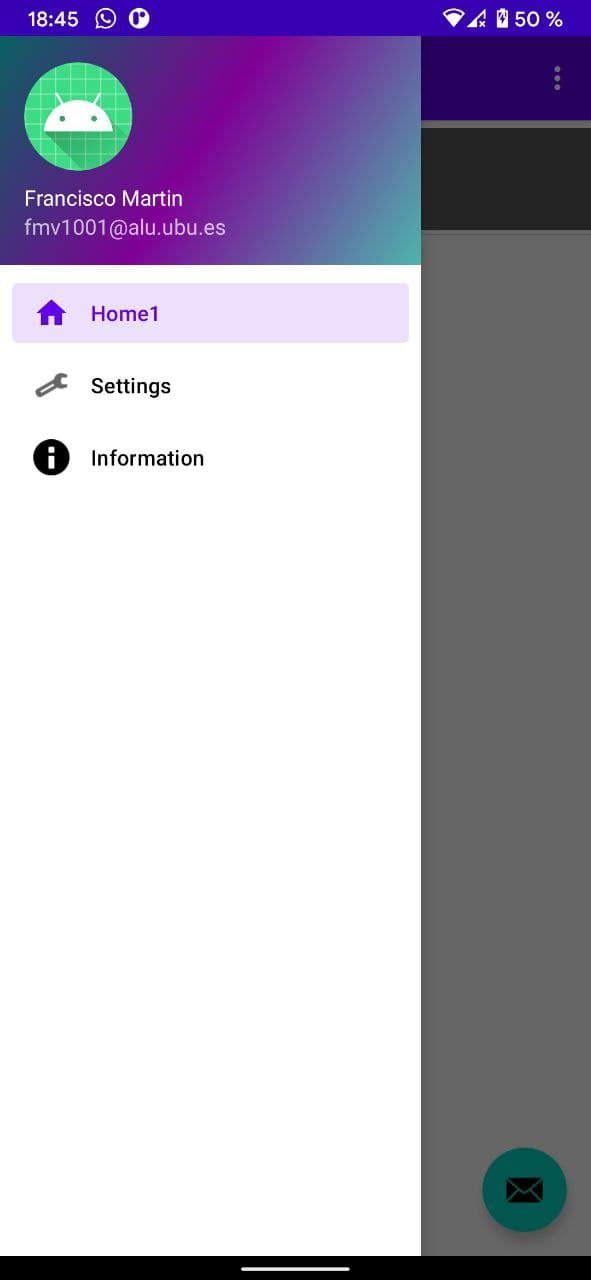
\includegraphics[width=0.35\linewidth]{img/appdevice}
	\caption{Aplicación ejecutada en dispositovo Android.}
	\label{fig:androapp}
\end{figure}
\end{enumerate}

\textbf{Generar APK de la aplicación}\\
Para generar el APK debemos realizar los siguientes pasos:
\begin{enumerate}
\item
	Primero debemos dirigirnos a la barra superior y ir al menú \textit{Build -> Generate Signed Bundle/APK}.
\imagen{asapk}{Menú Build de Android Studio para generar APK.}
\item
	Después, seleccionamos la opción APK y hacemos clic en \textit{Next}.
\imagen{asapk1}{Menú Build de Android Studio para generar APK.}
\item
	Después, seleccionamos la firma a usar o creamos una nueva desde \textit{Create new...} y hacemos clic en \textit{Next}.
\imagen{asapk3}{Menú \textit{Generate Signed Bundle/APK}.}
\imagen{asapk2}{Menú \textit{New key Store}.}
\item
	Después, seleccionamos \textit{release} y la opción \textit{V2 (Full APK Signature)} para que se cree el APK ya firmado, y hacemos clic en \textit{Finish}. Ahora sólo debemos esperar a que Gradle genere el archivo APK.
\imagen{asapk4}{Menú \textit{Generate Signed Bundle/APK}.}
\item
	Una vez generado lo podremos encontrar en la carpeta \textit{/AndroidApp/app/release/}
\end{enumerate}

Después de generar el archivo lo pasamos al teléfono y lo ejecutamos, misma salida que \ref{fig:androapp}.

\subsubsection{Ejecución del servidor}

Para la ejecución del servidor deberemos haber instalado previamente Visual Studio Code y Python 3 en el dispositivo que queramos desplegarlo.\\
Una vez instalados los componentes, abrimos Visual Studio Code, importamos el proyecto (tal como se explica en manual \ref{importtovsc}).
Después abrimos el archivo MainServer.py y en la esquina superior derecha ejecutamos pinchando el el icono \textit{play/run}. 
Seguidos estos pasos el servidor ya se encuentra en ejecución.
\imagen{runvsc}{Ejecución del servidor desde Visual Studio Code.}

También podemos ejecutar el servidor desde comandos situándonos en la carpeta \textit{/Server/} y desde el terminal ejecutamos el comando:\\
\textit{python3 MainServer.py}



\section{Pruebas del sistema}














\apendice{Documentación de usuario}

\section{Introducción}

En esta sección vamos a detallar los requisitos necesarios para la instalación y uso del sistema, así como el manual de cómo realizar dicha instalación. También se desarrollará un manual de uso. Todo ello enfocado al usuario final.

\section{Requisitos de usuarios}

\begin{itemize}
\item
	Dispositivo Android con una versión igual o superior a Android Jelly Bean o Android 4.1, para el uso de la aplicación.
\item
	Dispositivo de bajo consumo Raspberry Pi (recomendado) o PC con conexión a Internet, y con Python 3 instalado, para albergar el servidor.
\item
	Es necesario que el dispositivo Android y el dispositivo que vaya a ejecutar el servidor estén conectados a la misma WIFI.
\end{itemize}

\section{Instalación}

Para realizar la instalación del sistema, deberemos realizar dos instalaciones por separado, el servidor y la aplicación. Primero realizaremos la instalación del servidor ya que requiere algo más de tiempo.

\subsubsection{Instalación del servidor}

Esta instalación del servidor se realizará en un dispositivo de bajo consumo como es la Raspberry Pi, aunque si no se dispone de un dispositivo de estas características se puede saltar al paso \ref{paso10} y realizar la instalación en el PC.\\

\textbf{Requisitos}

\begin{itemize}
\item
	Raspberry Pi
\item
	Tarjeta SD de al menos 8 GB, ya que el sistema ocupa 4 GB de ellos.
\item
	Un PC con conexión a internet.
\item \label{piperifs}
	Un Monitor, ratón y teclado para usar la Raspberry Pi, nos vale cualquiera que tenga USB.
\end{itemize}

\textbf{Preparación de la Raspberry e instalación del servidor}\\

\begin{enumerate}
\item
	Insertamos la tarjeta SD en el PC.
\item
	Elegimos y descargamos el sistema operativo que queremos instalar en formato iso.
	Se recomienda el sistema operativo oficial, ya que es el sistema con el que se hacen las pruebas y para el que está diseñado. Lo encontramos en la página oficial, clic \href{https://www.raspberrypi.org/software/operating-systems/#raspberry-pi-os-32-bit}{aquí}.
	Pero también se pueden instalar otros sistemas si así se desea, aquí \cite{pios}.
	\imagen{raspdownload}{Página de descarga de Rasberry Pi OS.}
\item
	Una vez descargado el sistema operativo necesitamos una herramienta para instalar el sistema operativo en formato iso en la tarjeta SD.
	Se recomienda el uso de Raspberry Pi Imager, que podemos encontrarlo \href{https://www.raspberrypi.org/software/}{aquí}.
\item
	Cuando la herramienta este instalada, la abrimos y elegimos el archivo iso y el dispositivo de almacenamiento en el que queremos instalarlo (tarjeta SD).
	Pinchamos en \textit{write}.
\imagen{raspdownload1}{Herramienta Raspberry Pi Imager.}
\item
	Esperamos a que concluya el proceso y ya tenemos la tarjeta preparada.
\item
	Después de preparar la tarjeta la introducimos en el hueco dispuesto para ello de la Raspberry Pi. La conectamos a la corriente y a los periféricos necesarios ya mencionados en \ref{piperifs}.
\item
	Una vez instalado el sistema operativo siguiendo el instalador abrimos un terminal y ejecutamos el siguiente comando:\\
	\textit{python3 --version}\\
	Si el mensaje mostrado es \textit{Python X.X.X}, ya está instalado, pasar al siguiente paso.\\
	Si no ejecutamos el siguiente comando y esperamos a su instalación.
	
	\textit{sudo apt install python 3}
\item
	Cuando acabe la instalación ya tenemos la Raspberry preparada para ejecutar el servidor.
\item
	Ahora procedemos a descargar los archivos del servidor, que podremos descargarlos directamente desde Raspberry Pi en el \href{https://github.com/fmv1001/DomoCamera}{repositorio} o desde el PC y mediante un USB lo descargamos y lo pasamos a la Raspberry Pi.
\item
	Cuando tengamos los archivos del repositorio, sólo necesitaremos la carpeta \textit{Server}, los demás archivos pueden ser borrados. \label{paso10}
\item
	Después abrimos un terminal y nos colocamos dentro de la carpeta \textit{Server/logic}.
\item
	Es posible que haya que instalar las dependencias, OpenCV y SQLAlchemy, para python. Para ello ejecutamos en el terminal:\\
	\textit{pip3 install opencv-python}\\
	\textit{pip3 install SQLAlchemy}
\item
	Por último ejecutamos en el terminal el archivo \textit{MainServer.py}, y ya tendremos el servidor en funcionamiento. Para ello ejecutamos el siguiente comando:\\
	\textit{python3 MainServer.py}\\

\end{enumerate}

\subsubsection{Instalación de la app}

\begin{itemize}
\item
	En primero lugar descargamos los archivos, que podremos descargarlos directamente desde el dispositivo Android en el \href{https://github.com/fmv1001/DomoCamera}{repositorio} o desde el PC y mediante un USB lo descargamos y lo pasamos al smartphone.
	Este archivo que queremos es el archivo APK que se encuentra en la carpeta \textit{/AndroidApp/app/release/}.
\item
	Una vez descragado, lo debemos abrir en el dispositivo Android.
	Para ello nos dirigimos al almacenamiento del dispositivo donde hayamos guardado el archivo y lo abrimos.
\item
	Recibiremos un cuadro de diálogo (figura \ref{fig:appinstall}) que nos pregunta si queremos instalar la aplicación, debemos indicar \textit{instalar}.
\imagengrande{0.35}{appinstall}{Instalación de la aplicación desde un archivo APK.}
\item
	Es posible que recibamos un aviso como el que se muestra a continuación (figura \ref{fig:appinstall1}).
\imagengrande{0.35}{appinstall1}{Aviso en la instalación de la aplicación desde un archivo APK.}
	Debemos pulsar en \textit{Instalar de todas formas}.
\end{itemize}



\section{Manual del usuario}

En este manual se va a proceder a explicar cómo hacer uso de la aplicación.
En este enlace (\href{https://youtu.be/txAF8uAJ6B0}{Vídeo manual de usuario}), podremos ver este manual en formato vídeo.

\subsubsection{Conectarse al servidor}

Para conectarnos al servidor debemos navegar hasta la pantalla \textit{Settings}.

\begin{itemize}
\item
	Desde la pantalla principal abriremos el menú de navegación en el borde superior izquierdo (figura \ref{fig:manualuse0}).
	\imagengrande{0.35}{manualuse0}{Pantalla principal de la aplicación.}
\item
	Desde el menú de navegación pulsaremos \textit{Settings} para ir a la pantalla de \textit{Settings} (figura \ref{fig:manualuse01}).
	\imagengrande{0.35}{manualuse01}{Menú de navegación de la aplicación.}
\item
	Una vez en la pantalla de \textit{Settings} procederemos a rellenar los campos con la Ip del servidor y el puerto de escucha (este es el 8888 por defecto) (figura \ref{fig:manualuse1}).
	\imagengrande{0.35}{manualuse1}{Pantalla \textit{Settings} de la aplicación.}
\item
	Por último pulsamos en \textit{Conectarse con el servidor}.
\end{itemize}

\subsubsection{Añadir cámara}

Para añadir una cámara debemos situarnos en la pantalla principal y abrir el menú desplegable.

\begin{itemize}
\item
	Desde la pantalla principal abriremos el menú de desplegable en el borde superior derecho (figura \ref{fig:manualuse20}).
	\imagengrande{0.35}{manualuse20}{Pantalla principal de la aplicación.}
\item
	Desde el menú de desplegable pulsaremos \textit{Add camera} y nos saltará un cuadro de diálogo (figs. \ref{fig:manualuse21} y \ref{fig:manualuse3}).
	\imagengrande{0.35}{manualuse21}{Pantalla principal con menú desplegable abierto.}
	\imagengrande{0.35}{manualuse3}{Diálogo para añadir cámara en la aplicación.}
\item
	Una vez en cuadro de diálogo, rellenamos los campos exigidos y hacemos clic en aceptar (figura \ref{fig:manualuse4}).
	\imagengrande{0.35}{manualuse4}{Diálogo para añadir cámara en la aplicación.}
\item
	Se ha mostrado en la pantalla principal el botón de la cámara introducida (figura \ref{fig:manualuse5}).
	\imagengrande{0.35}{manualuse5}{Pantalla principal con cámara añadida en la aplicación.}
\end{itemize}

\subsubsection{Ver cámara}

Para ver una cámara debemos situarnos en la pantalla principal y debe haber alguna ya añadida anteriormente.

\begin{itemize}
\item
	Desde la pantalla principal pulsaremos el botón de la cámara que deseemos ver, están designadas con su nombre (figura \ref{fig:manualuse5a}).
	\imagengrande{0.35}{manualuse5a}{Pantalla principal con cámara añadida en la aplicación.}
\item
	Se nos abrirá una pantalla donde se muestra la imagen en teimpo real (figura \ref{fig:manualuse6}).
	\imagengrande{0.35}{manualuse6}{Pantalla de visualización de cámara.}
\item
	Si lo deseamos podemos tumbar el dispositivo para ver una imagen mas amplia (figura \ref{fig:manualuse7}).
	\imagengrande{0.9}{manualuse7}{Pantalla de visualización de cámara tumbada.}
\end{itemize}

\subsubsection{Grabar de la cámara}

Para grabar una pequeña secuencia de vídeo debemos encontrarnos en pantalla de visualización de una de las cámaras.

\begin{itemize}
\item
	Una vez en la pantalla de visualización, pinchamos en el botón gris y rojo (figura \ref{fig:manualuse61}).
	\imagengrande{0.35}{manualuse61}{Pantalla de visualización de cámara.}
\item
	Se grabará un vídeo que podremos ver en el almacenamiento del dispositivo.
\end{itemize}

\subsubsection{Eliminar cámara}

Para eliminar una cámara debemos situarnos en la pantalla principal y abrir el menú desplegable.

\begin{itemize}
\item
	Desde la pantalla principal abriremos el menú de desplegable en el borde superior derecho (figura \ref{fig:manualuse20a}).
	\imagengrande{0.35}{manualuse20a}{Pantalla principal de la aplicación.}
\item
	Desde el menú de desplegable pulsaremos \textit{Delete camera} y nos saltará un cuadro de diálogo (figura \ref{fig:manualuse80}).
	\imagengrande{0.35}{manualuse80}{Pantalla principal con menú desplegable abierto.}
\item
	Una vez en cuadro de diálogo, escogemos la cámara para eliminar y hacemos clic en aceptar (figura \ref{fig:manualuse81}).
	\imagengrande{0.35}{manualuse81}{Diálogo para eliminar cámara en la aplicación.}
\item
	Se ha eliminado de la pantalla principal el botón de la cámara (figura \ref{fig:manualuse}).
	\imagengrande{0.35}{manualuse}{Pantalla principal con cámara eliminada en la aplicación.}
\end{itemize}

\subsubsection{Desconectarse del servidor}

Para desconectarse del servidor debemos situarnos en la pantalla principal y abrir el menú desplegable.

\begin{itemize}
\item
	Desde la pantalla principal abriremos el menú de desplegable en el borde superior derecho (figura \ref{fig:manualuse20b}).
	\imagengrande{0.35}{manualuse20b}{Pantalla principal de la aplicación.}
\item
	Desde el menú de desplegable pulsaremos \textit{Disconnect} (figura \ref{fig:manualuse90}).
	\imagengrande{0.35}{manualuse90}{Pantalla principal con menú desplegable abierto.}
\end{itemize}

\subsubsection{Parar servidor}

Para parar el servidor debemos situarnos en la pantalla principal y abrir el menú desplegable.

\begin{itemize}
\item
	Desde la pantalla principal abriremos el menú de desplegable en el borde superior derecho (figura \ref{fig:manualuse20c}).
	\imagengrande{0.35}{manualuse20c}{Pantalla principal de la aplicación.}
\item
	Desde el menú de desplegable pulsaremos \textit{Stop Server} (figura \ref{fig:manualuse91}).
	\imagengrande{0.35}{manualuse91}{Pantalla principal con menú desplegable abierto.}
\end{itemize}

\subsubsection{Visualizar log}

Para visualizar el log debemos navegar hasta la pantalla \textit{Log}.

\begin{itemize}
\item
	Desde la pantalla principal abriremos el menú de navegación en el borde superior izquierdo.
	\imagengrande{0.35}{manualuse0a}{Pantalla principal de la aplicación.}
\item
	Desde el menú de navegación pulsaremos \textit{Log} para ir a la pantalla de \textit{Log} (figura \ref{fig:manualuse02}).
	\imagengrande{0.35}{manualuse02}{Menú de navegación de la aplicación.}
\item
	Una vez en la pantalla de \textit{Log} podemos ver el log y hacer scroll sobre él (figura \ref{fig:manualuselog}).
	\imagengrande{0.35}{manualuselog}{Pantalla \textit{Log} de la aplicación.}
\end{itemize}





\bibliographystyle{IEEEtran}
\bibliography{IEEEabrv,bibliografiaAnexos}

\end{document}
